\section{Lezione 15} \hfill 01/04/2026\\
Il taglio saltuario può essere realizzato anche nella pecceta pura, pur essendo piuttosto raro.\\
In Europa viene molto trattato con la selvicoltura industriale: 
\begin{itemize}[nosep]
    \item i rimboschimenti vengono fatti con 2000-2500 piantine ad ettaro;
    \item normalmente i turni sono compresi tra i 70 ed i 90 anni;
    \item le cure colturali consistono solitamente in uno sfollo entro i 10-15 anni (entro i 10 m di altezza) e due diradamenti (entro i 40-50 anni);
    \item si vuole raggiungere le 300-500 piante ad ettaro, con un diametro obiettivo di 30 cm (minimo) o 40 cm.
\end{itemize}
Gli svedesi, che lavorano soprattutto in piano, chiamano il primo sfollo un ``diradamento non commerciale''; il successivo taglio viene fatto con l'harvester, mediante un diradamento selettivo.\\
Le cure culturali, nell'abete rosso e soprattutto negli impianti artificiali, sono essenziali per la stabilità.
\begin{figure}[htbp]
     \centering
     % Prima Immagine
     \begin{subfigure}[b]{0.33\textwidth}
         \centering
         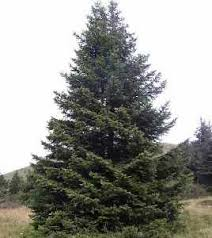
\includegraphics[width=\textwidth]{immagini/abete_rosso_portamento.jpg}
        %\caption{}
     \end{subfigure}
     \hfill % Spazio elastico tra le immagini
     % Seconda Immagine
     \begin{subfigure}[b]{0.3\textwidth}
         \centering
         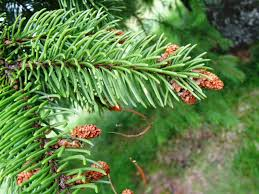
\includegraphics[width=\textwidth]{immagini/abete_rosso_foglie.jpg}
        %\caption{}
     \end{subfigure}
     \hfill % Spazio elastico tra le immagini
     % Terza Immagine
     \begin{subfigure}[b]{0.33\textwidth}
         \centering
         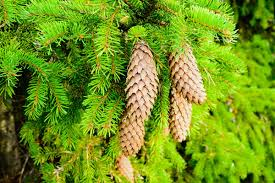
\includegraphics[width=\textwidth]{immagini/abete_rosso_coni.jpg}
        %\caption{}
     \end{subfigure}
    \caption{Abete rosso}
     \label{fig:abete_rosso}
\end{figure}
\subsubsection{I diradamenti}
Un diradamento serve per:
\begin{itemize}[nosep]
    \item scegliere delle piante che si vuole che arrivino a fine turno;
    \item aumentare la stabilità del popolamento (robustezza).
\end{itemize}
Subito dopo che viene svolto un diradamento, per un certo periodo il popolamento è tendenzialmente più instabile (3-5 anni). Questo perché si va a sfasare l'equilibrio di facilitazione che si era creato tra le diverse piante.\\
I diradamenti si basano su 4 parametri, interconnessi tra di loro (tipo, grado, frequenza ed epoca di inizio):
\begin{itemize}[nosep]
    \item tipo, parametro che da il nome al diradamento:
    \begin{enumerate}[nosep]
        \item scelta delle piante a priori (detti sistematici, geometrici), ovvero il criterio di diradamento viene scelto prima se le piante sono tutte uguali (diventa indifferente il taglio di una pianta rispetto ad un'altra); conviene quasi sempre fare tagli nord-sud, e di traverso (poiché rimuovono più spazio tagliando meno piante). Si può fare un'eccezione al taglio geometrico per una pianta (``diradamento con il salto");
        \item scelta delle piante a posteriori: la scelta viene fatta quando si entra in bosco. I criteri di scelta possono essere a negativo (si rimuovono le piante brutte, fatti maggiormente in passato) o a positivo (si mantengono le piante belle). I diradamenti negativi possono essere dal basso (operano sul piano dominato, es. rimozione di tutti gli alberi con diametro inferiore a quello medio), dall'alto (eliminazione delle piante con i difetti, nel piano dominante) e misti (combinazione dei diradamenti dal basso e dall'alto). Il criterio positivo consiste nell'andare in bosco e scegliere i candidati migliori (eliminando così i relativi concorrenti).\\
        Gli alberi indifferenti non sono ne i candidati e ne i relativi concorrenti, sono quelli che alleveranno i candidati. Il numero di candidati da scegliere può essere il valore finale del bosco che voglio ottenere, oppure effettuo una programmazione dei diradamenti. I concorrenti sono piante belle, perché sono in grado di concorrere alla competizione contro i candidati. 
    \end{enumerate}
    \item grado: indica l'intensità del diradamento (``quanti alberi taglio?"). Si basa sulla copertura delle chiome e non sulla densità di rimozione: l'isolamento degli alberi è un diradamento forte, se non si isolano gli alberi è un diradamento debole.\\
    Un diradamento di tipo selettivo (ovvero con selezione positiva) è un diradamento forte, perché deve liberare la chioma. Un diradamento dal basso solitamente è un diradamento debole, perché riguarda le piante sotto copertura.\\
    Solitamente è meglio un diradamento forte, per ragioni economiche. 
    \item frequenza: i diradamenti possono essere frequenti (intervallo tra i diradamenti inferiore ad un decimo del tempo del turno) o poco frequenti (intervallo tra i diradamenti maggiore del decimo del tempo del turno). 
    \item epoca d'inizio: in funzione dello stadio del popolamento, possono essere precoci (prima della perticaia) o tardivi (dopo la perticaia). Nella perticaia c'è il culmine dell'incremento in altezza della pianta (maggiore crescita). Solitamente conviene fare i diradamenti precoci, in modo che si possa avere maggiore influenza rispetto che alla natura.
\end{itemize}
Si può sapere che è ora di fare un diradamento, osservando:
\begin{itemize}[nosep]
    \item il rapporto di snellezza (h/b, con la stessa unità di misura), per l'abete rosso:
    \begin{enumerate}[nosep]
        \item se è superiore a 100 la pianta è molto instabile;
        \item se è tra 80 e 100 la pianta è instabile;
        \item se inferiore ad 80 è stabile.
    \end{enumerate} 
    Alcune latifoglie possono essere molto snelle e robuste.
    \item la profondità di chioma: se la chioma scende a più di metà del fusto, la pianta è molto stabile. Se la chioma è concentrata nell'ultimo terzo, è molto instabile. Se è nel mezzo occorre fare un diradamento.
\end{itemize}
Se il rapporto di snellezza del popolamento di abete rosso è superiore a 100, conviene fare un taglio raso (e far ricominciare da capo la successione) o non fare nulla (la rimozione di una pianta può avere un effetto domino con gli altri individui).\\
Quando si è tra 80 e 100, si può intervenire con un diradamento che tenga in considerazione gruppi di alberi, e non il singolo albero. Nel piano subalpino la struttura del popolamento è a collettivi: anche quando il bosco è chiuso, certe piante sono maggiormente in relazione tra di loro, rispetto ad altre piante (considerate come unità selvicolturale, es. 5-6 piante). Il diradamento potrebbe dare il contorno alla unita selvicolturale.\\
Se il popolamento è stabile, il diradamento migliore è il selettivo o libero, in modo da eliminare gli individui (concorrenti) che si vogliono.\\
Il diradamento dal basso è un taglio che ha poco effetto: infatti, si vanno ad eliminare le piante che hanno perso la competizione, e che di fatto sono già morte.\\
Nelle Alpi solitamente si fa un diradamento selettivo (perché si vuole ottenere la qualità); in Svezia invece si vuole ottenere la maggiore quantità (dovendo fare prevalentemente carta).
\subsection{Picio-abieteti, Picio-abeto-faggeti}
Il faggio, abete bianco e rosso hanno delle caratteristiche ecologiche simili.\\
Tipici del piano montano, nella regione esalpica o mesalpica.\\
Gli areali sono abbastanza sovrapponibili (tranne nell'Appennino dove l'abete rosso non c'è), e pertanto potrebbero creare boschi misti. In Appennino sono fondamentalmente di abete bianco e faggio, mentre nelle Alpi potrebbero essere tutti e tre assieme.\\
In Europa, questi boschi dovrebbero essere molto piú presenti di quanto non lo siano: questo perché l'uomo ha favorito l'abete rosso più delle altre specie.\\
Normalmente, il comportamento di queste specie in natura è di sostituzione: le specie si alternano, con fasi di dominanza alterne. L'abete bianco difficilmente si rinnova sotto se stesso, il faggio invece riesce.\\
Per i selvicoltori è difficile sbagliare lavorando con questi popolamenti, perché almeno una delle tre specie resiste.\\
Il trattamento ideale di questo popolamento misto è il taglio saltuario: con un periodo di curazione di 10-20 anni (rispettivamente se la crescita é veloce o lenta). Si entra in bosco tagliando gli alberi che hanno raggiunto il diametro obiettivo, facendo le eventuali cure culturali sulle piante giovani. Questo sistema è molto costoso, perché si devono fare molti cantieri per portare fuori poca biomassa. Per decenni è stato il sistema perfetto per i forestali, inventato in Svizzera (foret-giardinee), ed oggi è stato quasi del tutto abbandonato.\\
Conviene creare un popolamento disetaneo ad unità selvicolturali, e non a piede d'albero. Esiste il concreto rischio della coetanizzazione del bosco, sia dal basso (generazione di rinnovazione che si alza tutta assieme) che dall'alto (il taglio è ridotto e la copertura diventa eccessiva). 
\subsection{Piano montano e subalpino}
Si trova ancorar l'abete rosso subalpino.\\
Si possono trovare le ontanete di ontano verde (popolamento azonale). L'ontano verde:
\begin{itemize}[nosep]
    \item cresce in forma arbustiva;
    \item viene poco utilizzato in selvicoltura;
    \item è un indicatore della presenza dell'acqua (es. fontanivi);
    \item essendo elastica influenza la caduta della neve al suolo (nessuna protezione contro le valanghe);
    \item in passato usato dai malgari come legna da ardere (spesso piantato lungo le mulattiere, per facilitare la raccolta).
\end{itemize}  
Possono essere dei tipi ad ontano verde e larice.\\
Un altro popolamento del piano montano e subalpino è il popolamento delle pinete di pino montano.\\
Con pino montano (la cui tassonomia è ancora in discussione) vengono descritti tre pini diversi:
\begin{itemize}[nosep]
    \item pino uncinato: ad ovest delle Alpi, è di terza grandezza (massimo 20 metri), arboreo, con i coni che hanno gli unboni ad uncino;
    \item pino mugo: ad est delle Alpi, di norma rimane un arbusto (non diventa un albero), può anche essere policornico e non ha capacità pollonifera;
    \item Pinus pumila, in mezzo ai due areali e con caratteristiche intermedie tra le due. 
\end{itemize} 
\subsubsection{Pino uncinato - Pinus uncinata}
Colonizzatore delle peggiori stazioni, su substrati sterili. Riesce ad ibridarsi con il pino silvestre, e nelle zone a contatto possono esserci ibridi.\\
Ha una funzione di protezione e forma boschi primitivi.
\begin{figure}[htbp]
     \centering
     % Prima Immagine
     \begin{subfigure}[b]{0.33\textwidth}
         \centering
         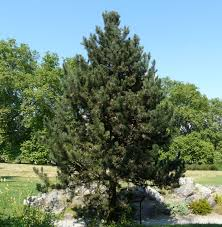
\includegraphics[width=\textwidth]{immagini/pino_uncinato_portamento.jpg}
        %\caption{}
     \end{subfigure}
     \hfill % Spazio elastico tra le immagini
     % Seconda Immagine
     \begin{subfigure}[b]{0.3\textwidth}
         \centering
         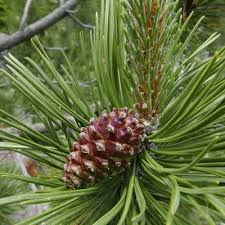
\includegraphics[width=\textwidth]{immagini/pino_uncinato_foglie.jpg}
        %\caption{}
     \end{subfigure}
     \hfill % Spazio elastico tra le immagini
     % Terza Immagine
     \begin{subfigure}[b]{0.33\textwidth}
         \centering
         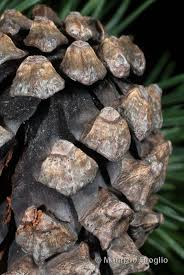
\includegraphics[width=\textwidth]{immagini/pino_uncinato_cono.jpg}
        %\caption{}
     \end{subfigure}
    \caption{Pino uncinato}
     \label{fig:pino_uncinato}
\end{figure}
\subsubsection{Pino mugo - Pinus mugo}
Essendo un pino è una specie pioniera, in grado di arrivare fino al limite del bosco, allungandosi fino a fondo valle.\\
Al contrario del pino silvestre, il pino mugo non sopporta l'inghiaiamento: una frana non colonizzata dal pino mugo, indica che la frana è ancora in movimento.\\
Oggi non viene quasi fatta selvicoltura con il pino mugo, in passato veniva fatta per la legna da ardere. In Alto Adige, c'è l'uso tradizionale di estrarre dalle foglie il mugoglio (sia per la farmaceutica che per la cosmetica), facendo tagli a scacchiera.\\
È presente solamente nelle Alpi orientali, e le mughete sono protette nelle aree Natura 2000. Sono un problema nei pascoli abbandonati (regione esalpica), perchè gli ha invasi: è un aspetto negativo se uno vuole tornare al pascolo.
\begin{figure}[htbp]
     \centering
     % Prima Immagine
     \begin{subfigure}[b]{0.33\textwidth}
         \centering
         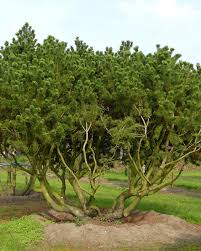
\includegraphics[width=\textwidth]{immagini/pino_mugo_portamento.jpg}
        %\caption{}
     \end{subfigure}
     \hfill % Spazio elastico tra le immagini
     % Seconda Immagine
     \begin{subfigure}[b]{0.3\textwidth}
         \centering
         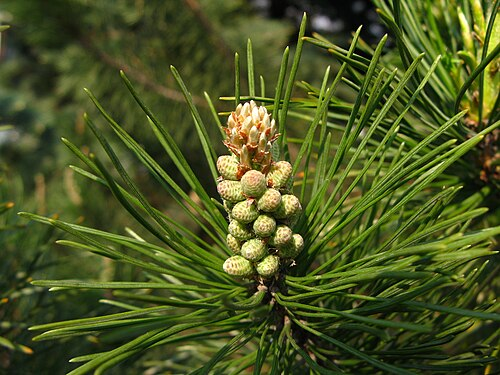
\includegraphics[width=\textwidth]{immagini/pino_mugo_foglie.jpg}
        %\caption{}
     \end{subfigure}
     \hfill % Spazio elastico tra le immagini
     % Terza Immagine
     \begin{subfigure}[b]{0.33\textwidth}
         \centering
         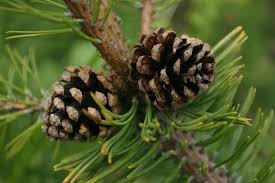
\includegraphics[width=\textwidth]{immagini/pino_mugo_coni.jpg}
        %\caption{}
     \end{subfigure}
    \caption{Pino mugo}
     \label{fig:pino_mugo}
\end{figure}
\subsubsection{Larice - Larix decidua}
Anche detto ``larice europeo". È un relitto delle glaciazioni, poiché spinto a sud dai ghiacciai; con il loro ritiro, il larice è rimasto nelle Alpi, nei Carpazi, nei Sudeti ed in Polonia.\\
Si trova nel piano subalpino.\\
Oltre gli Urali, ci sono altri larici: Larix sibirica, Larix dahurica, Larix gmelinii. In Canada/USA c'è il Larix laricina. Inoltre, c'è il Larice coreano, giapponese...\\
È una strana specie, perché ha un comportamento misto tra pioniera e definitiva:
\begin{itemize}[nosep]
    \item rapido accrescimento (relativo al piano subalpino);
    \item apparato radicale fittonante;
    \item adora i suoli minerali;
    \item fortemente eliofilo;
    \item ha bisogno di presenza di acqua, perchè è un grande traspiratore (funziona come fosse una latifoglia);
    \item ha una vita lunghissima (può superare i 1000 anni);
    \item è per eccellenza una specie microterma;
    \item gli servono solo 15 gg per svolgere il suo ciclo vegetativo;
    \item riesce a salire fino al limite del bosco (2300-2500 m sulle Alpi);
    \item assieme al cembro ed al pino mugo, costituisce il popolamento al limite del bosco;
    \item può scendere fino a 1000 m di quota (si comporta da pioniera e verrà successivamente rimossa);
    \item normalmente forma popolamenti pionieri;
    \item rispetto alla neve, non è un grande protettore dai suoi movimenti (poiché perde la chioma d'inverno e non interrompe il manto nevoso);
    \item Coleophora e Zeiraphera griseana che sono dei defogliatori, con gradazioni cicliche ogni 8-10 anni (ad agosto);
    \item soggetto a cancro del larice, che forma delle curvature del fusto. 
\end{itemize}
\begin{figure}[htbp]
     \centering
     % Prima Immagine
     \begin{subfigure}[b]{0.33\textwidth}
         \centering
         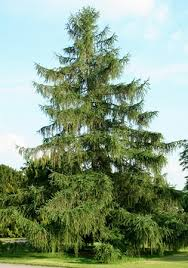
\includegraphics[width=\textwidth]{immagini/larice_portamento.jpg}
        %\caption{}
     \end{subfigure}
     \hfill % Spazio elastico tra le immagini
     % Seconda Immagine
     \begin{subfigure}[b]{0.3\textwidth}
         \centering
         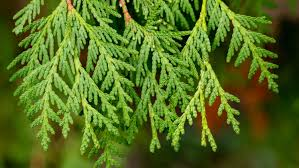
\includegraphics[width=\textwidth]{immagini/larice_foglie.jpg}
        %\caption{}
     \end{subfigure}
     \hfill % Spazio elastico tra le immagini
     % Terza Immagine
     \begin{subfigure}[b]{0.33\textwidth}
         \centering
         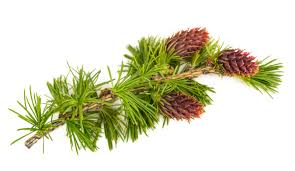
\includegraphics[width=\textwidth]{immagini/larice_coni.jpg}
        %\caption{}
     \end{subfigure}
    \caption{Larice}
     \label{fig:larice}
\end{figure}